\documentclass[border=10pt]{standalone}

\usepackage{tikz}
\usepackage{tikzsymbols}
\usetikzlibrary{calc,patterns,shapes.geometric}

\def\centerarc[#1](#2)(#3:#4:#5){\draw[#1] ($(#2)+({#5*cos(#3)},{#5*sin(#3)})$) arc (#3:#4:#5);}

\begin{document}
	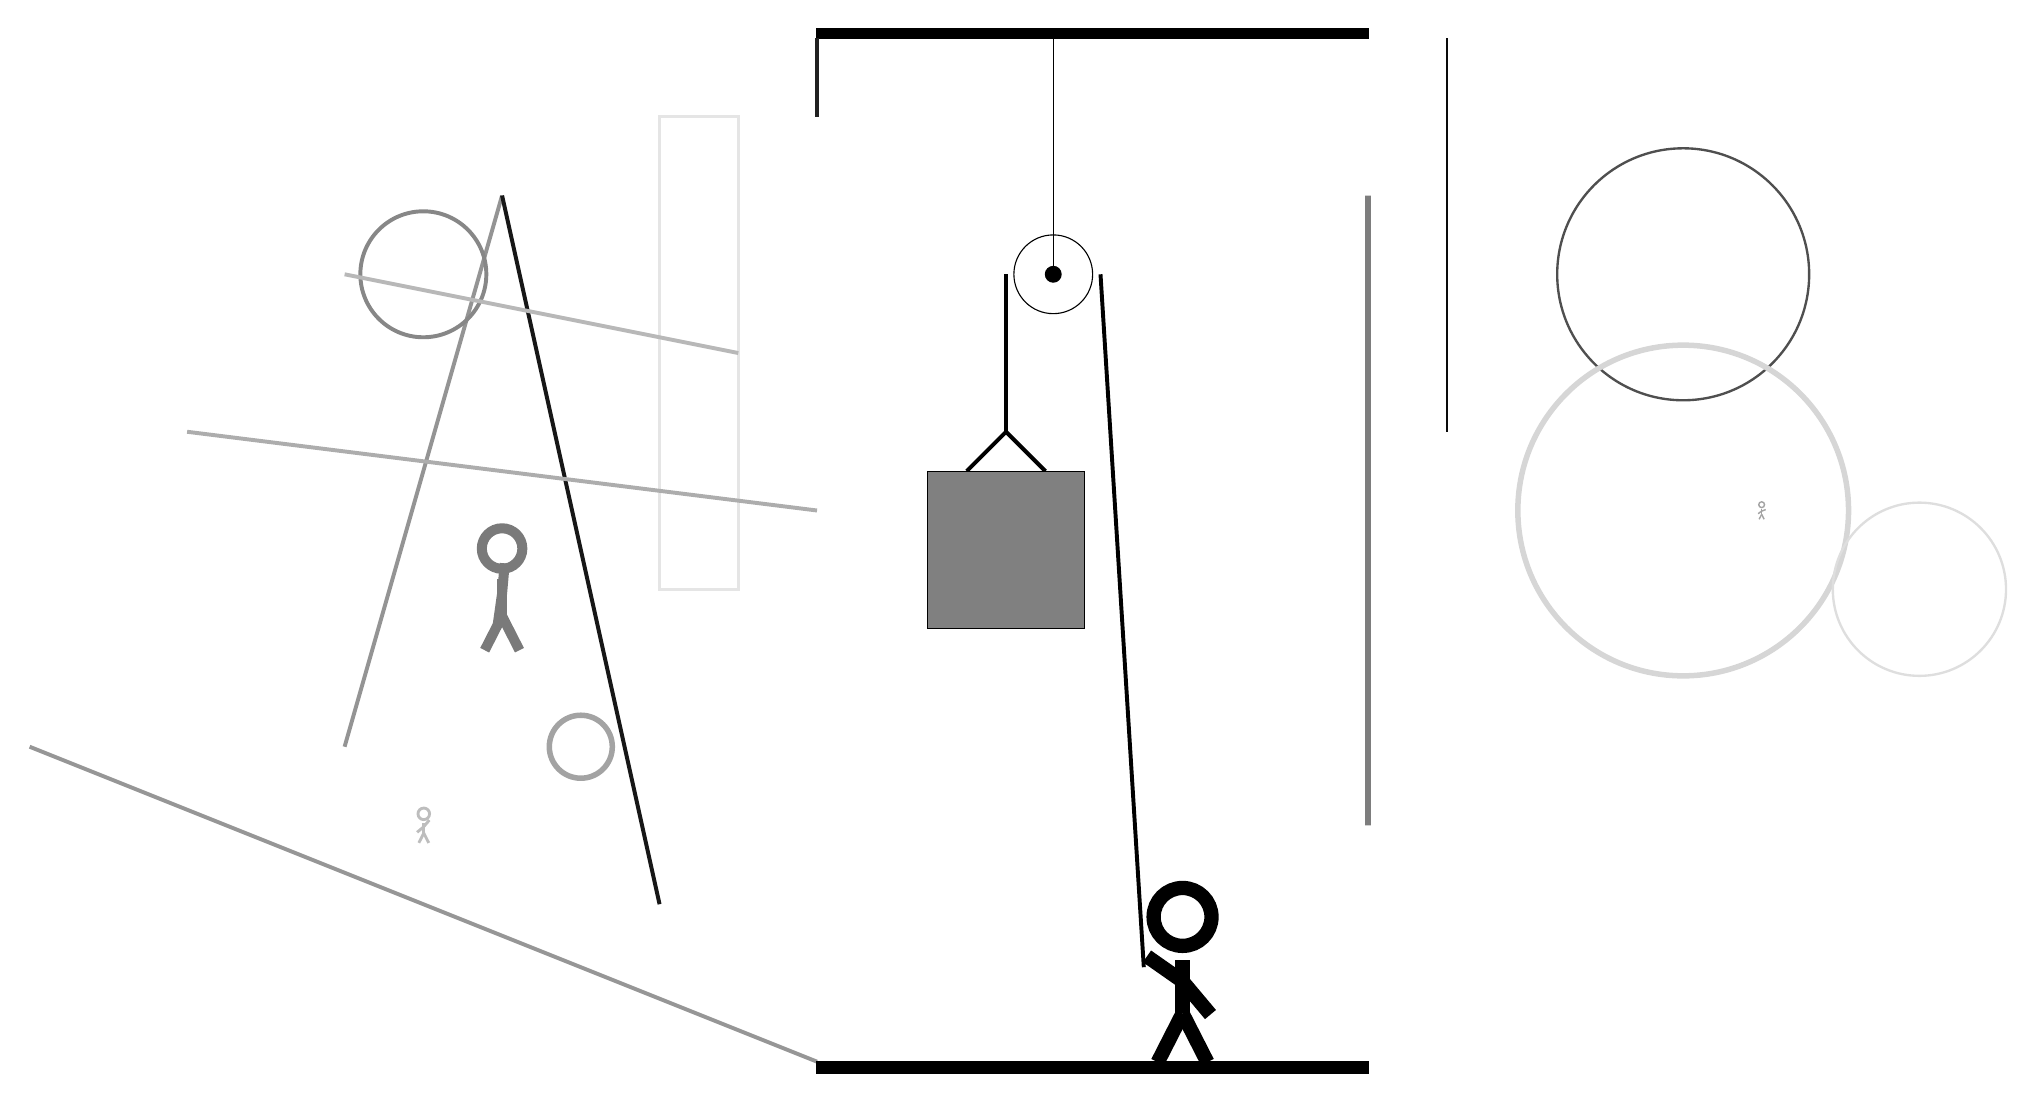
\begin{tikzpicture}
		%%%%% START %%%%%
		
		\draw[fill=black] (-2, 10) rectangle (5, 10.125);
		
		\draw (1, 7) circle (0.5);
		\draw[fill=black] (1, 7) circle (0.1);
		\draw (1, 10) -- (1, 7);
		
		\draw[line width=0.5mm] (-0.1, 4.5) -- (0.4, 5.0) -- (0.9, 4.5);
		\draw[fill=black!50] (-0.6, 4.5) rectangle (1.4, 2.5);
		
		\draw[line width=0.5mm] (0.4, 7) -- (0.4, 5.0);
		\centerarc[line width=0.5mm](1, 7)(0:180:0.6);
		\draw[line width=0.5mm](1.6, 7) -- (2.15, -1.8);
		
		\node at (2.6, -1.9) {\Strichmaxerl[10][-35][-50]};
		
		\draw[line width=0.3mm, color=black!96] (6, 10) rectangle (6, 5);
		
		\draw[line width=0.7mm, color=black!51] (5, 0) rectangle (5, 8);
		\draw[line width=0.5mm, color=black!41](-2, -3) -- (-12, 1);
		\draw[line width=0.5mm, color=black!42](-6, 8) -- (-8, 1);
		\draw [line width=0.3mm, color=black!69](9, 7) circle (1.6);
		
		\draw [line width=0.7mm, color=black!16](9, 4) circle (2.1);
		\draw [line width=0.5mm, color=black!47](-7, 7) circle (0.8);
		\draw [line width=0.3mm, color=black!13](12, 3) circle (1.1);
		\node[line width=0.6mm, color=black!36] at (10, 4) {\Strichmaxerl[1][36][21]};
		
		\draw [line width=0.7mm, color=black!36](-5, 1) circle (0.4);
		\draw[line width=0.6mm, color=black!87] (-2, 10) rectangle (-2, 9);
		\node[line width=0.6mm, color=black!52] at (-6, 3) {\Strichmaxerl[7][82][85]};
		\draw[line width=0.4mm, color=black!10] (-3, 9) rectangle (-4, 3);
		
		\draw[line width=0.5mm, color=black!91](-6, 8) -- (-4, -1);
		\node[line width=0.2mm, color=black!26] at (-7, 0) {\Strichmaxerl[2][40][50]};
		\draw [line width=0.4mm, color=black!56](-4, 8) circle (0.0);
		
		\draw[line width=0.5mm, color=black!28](-3, 6) -- (-8, 7);
		\draw[line width=0.5mm, color=black!32](-2, 4) -- (-10, 5);
		
		\draw[fill=black] (-2, -3) rectangle (5, -3.15);
		
		%%%%% END %%%%%
	\end{tikzpicture}
\end{document}